\documentclass[a4paper]{article}
\usepackage{amsmath, amsthm, amssymb, bm, graphicx, hyperref, mathrsfs}
\usepackage{booktabs}
\usepackage{graphicx}
\usepackage{float}    % 提供 H 位置选项
\usepackage[affil-it]{authblk}
\usepackage[backend=bibtex,style=numeric]{biblatex}

\usepackage{geometry}
\geometry{margin=1.5cm, vmargin={0pt,1cm}}
\setlength{\topmargin}{-1cm}
\setlength{\paperheight}{29.7cm}
\setlength{\textheight}{25.3cm}

\addbibresource{citation.bib}

\begin{document}
% =================================================
\title{Numerical Analysis Homework 3}

\author{Yilin Chen 3230101092
  \thanks{Electronic address: \texttt{yilinchen@zju.edu.cn}}}
\affil{(Numerical Analysis, Math2301), Zhejiang University }


\date{Due time:2025/11/13 \today}

\maketitle

% \begin{abstract}
%     The abstract is not necessary for the theoretical homework, 
%     but for the programming project, 
%     you are encouraged to write one.      
% \end{abstract}





% ============================================
\section*{I. Cubic Spline Determination}

Let \( p(x) = a x^3 + b x^2 + c x + d \). From \( s(0) = p(0) = 0 \), we obtain:
\[
d = 0.
\]

At the knot \( x = 1 \), we require continuity of function value, first derivative, and second derivative:
\begin{align*}
p(1) &= (2-1)^3 = 1, \\
p'(1) &= \frac{d}{dx}(2-x)^3 \bigg|_{x=1} = -3, \\
p''(1) &= \frac{d^2}{dx^2}(2-x)^3 \bigg|_{x=1} = 6.
\end{align*}

Compute derivatives of \( p \):
\[
p'(x) = 3a x^2 + 2b x + c, \quad p''(x) = 6a x + 2b.
\]

Substitute the conditions at \( x = 1 \):
\begin{align*}
a + b + c &= 1, \\
3a + 2b + c &= -3, \\
6a + 2b &= 6.
\end{align*}

$$\implies a = 7, \quad b = -18, \quad c = 12.$$

Thus,
\[
p(x) = 7x^3 - 18x^2 + 12x.
\]

Since \( s''(0) = p''(0) = 6a \cdot 0 + 2b = -36 \neq 0 \), \( s(x) \) is not a natural cubic spline.


\section*{II. Quadratic Spline Interpolation}

\subsection*{II-a}

A quadratic spline \( s \in \mathbb{S}_2^1 \) on \([a, b]\) with nodes \( a = x_1 < x_2 < \cdots < x_n = b \) consists of \( n-1 \) quadratic polynomials \( p_i \) on each interval \([x_i, x_{i+1}]\). Each \( p_i \) has 3 parameters, giving a total of \( 3(n-1) \) parameters. The conditions are:
\begin{itemize}
    \item Interpolation: \( p_i(x_i) = f_i \) and \( p_i(x_{i+1}) = f_{i+1} \) for \( i = 1, \dots, n-1 \), yielding \( 2(n-1) \) conditions.
    \item Continuity of first derivative at interior nodes: \( p_{i-1}'(x_i) = p_i'(x_i) \) for \( i = 2, \dots, n-1 \), yielding \( n-2 \) conditions.
\end{itemize}
Total conditions: \( 2(n-1) + (n-2) = 3n - 4 \). Since \( 3(n-1) = 3n - 3 \), there is one degree of freedom. Hence, an additional condition is needed to determine \( s \) uniquely.

\subsection*{II-b}

Let \( p_i(x) = A_i (x - x_i)^2 + B_i (x - x_i) + C_i \). The conditions are:
\begin{align*}
    p_i(x_i) &= C_i = f_i, \\
    p_i'(x_i) &= B_i = m_i, \\
    p_i(x_{i+1}) &= A_i (\Delta x_i)^2 + m_i \Delta x_i + f_i = f_{i+1}, \quad \text{where } \Delta x_i = x_{i+1} - x_i.
\end{align*}
Solving for \( A_i \):
\[
A_i = \frac{f_{i+1} - f_i - m_i \Delta x_i}{(\Delta x_i)^2}.
\]
Thus,
\[
p_i(x) = f_i + m_i (x - x_i) + \frac{f_{i+1} - f_i - m_i \Delta x_i}{(\Delta x_i)^2} (x - x_i)^2.
\]

\subsection*{II-c}

Given \( m_1 = f'(a) \), we use the continuity of the first derivative at interior nodes. For \( i = 2, \dots, n-1 \):
\[
p_{i-1}'(x_i) = p_i'(x_i).
\]
From part (b), on \([x_{i-1}, x_i]\):
\[
p_{i-1}'(x) = 2A_{i-1}(x - x_{i-1}) + m_{i-1}, \quad \text{with } A_{i-1} = \frac{f_i - f_{i-1} - m_{i-1} \Delta x_{i-1}}{(\Delta x_{i-1})^2}.
\]
At \( x = x_i \):
\[
p_{i-1}'(x_i) = 2 \cdot \frac{f_i - f_{i-1} - m_{i-1} \Delta x_{i-1}}{\Delta x_{i-1}} + m_{i-1} = \frac{2(f_i - f_{i-1})}{\Delta x_{i-1}} - m_{i-1}.
\]
Since \( p_i'(x_i) = m_i \), we obtain:
\[
m_i = \frac{2(f_i - f_{i-1})}{\Delta x_{i-1}} - m_{i-1}, \quad \text{for } i = 2, \dots, n-1.
\]
Starting from \( m_1 \), we can compute \( m_2, m_3, \ldots, m_{n-1} \) recursively.


\section*{III. Natural Cubic Spline Construction}

Let \( s_2(x) = A x^3 + B x^2 + C x + D \). The conditions are:

By continuity at \( x = 0 \):
\begin{align}
s_1(0) &= s_2(0) \implies 1 + c = D, \\
s_1'(0) &= s_2'(0) \implies 3c = C, \\
s_1''(0) &= s_2''(0) \implies 6c = 2B \implies B = 3c.
\end{align}

By natural boundary condition at \( x = 1 \):
\begin{align}
s_2''(1) = 6A + 2B = 6A + 6c = 0 \implies A = -c.
\end{align}

Thus,
\[
s_2(x) = -c x^3 + 3c x^2 + 3c x + (1 + c).
\]

\subsection*{Additional condition \( s(1) = -1 \):}
\[
s_2(1) = -c + 3c + 3c + 1 + c = 6c + 1 = -1 \implies c = -\frac{1}{3}.
\]

\section*{IV. Natural Cubic Spline and Bending Energy}

\subsection*{IV-a}

Let
\[
s(x) = 
\begin{cases}
s_1(x) = a_1 x^3 + b_1 x^2 + c_1 x + d_1 & \text{for } x \in [-1, 0], \\
s_2(x) = a_2 x^3 + b_2 x^2 + c_2 x + d_2 & \text{for } x \in [0, 1].
\end{cases}
\]
Given \( f(-1) = 0 \), \( f(0) = 1 \), \( f(1) = 0 \), the conditions are:
$$s_1(-1) = 0, \quad s_1(0) = 1, \quad s_2(0) = 1, \quad s_2(1) = 0, \quad s_1'(0) = s_2'(0), \quad s_1''(0) = s_2''(0), \quad s_1''(-1) = 0, \quad s_2''(1) = 0$$

Solving the equations gives:
\[
a_1 = -\frac{1}{2}, \quad b_1 = -\frac{3}{2}, \quad c_1 = 0, \quad a_2 = \frac{1}{2}, \quad b_2 = -\frac{3}{2}, \quad c_2 = 0.
\]
Thus,
\[
s(x) = 
\begin{cases}
1 - \frac{1}{2}x^3 - \frac{3}{2}x^2 & \text{for } x \in [-1, 0], \\
1 + \frac{1}{2}x^3 - \frac{3}{2}x^2 & \text{for } x \in [0, 1].
\end{cases}
\]

\subsection*{IV-b}

The bending energy is \( E(g) = \int_{-1}^{1} [g''(x)]^2  dx \).

For the natural cubic spline \( s \):

$$s_1''(x) = -3x - 3, \quad s_2''(x) = 3x - 3$$

Thus

$$E(s) = \int_{-1}^{0} (-3x-3)^2  dx + \int_{0}^{1} (3x-3)^2  dx = 6$$

(i) For the quadratic interpolant \( q(x) = 1 - x^2 \):
\[
q''(x) = -2, \quad E(q) = \int_{-1}^{1} (-2)^2  dx = 4 \cdot 2 = 8.
\]

(ii) For \( f(x) = \cos\left(\frac{\pi}{2}x\right) \):
\[
f''(x) = -\frac{\pi^2}{4} \cos\left(\frac{\pi}{2}x\right), \quad [f''(x)]^2 = \frac{\pi^4}{16} \cos^2\left(\frac{\pi}{2}x\right),
\]
\[
E(f) = \frac{\pi^4}{16} \int_{-1}^{1} \cos^2\left(\frac{\pi}{2}x\right) dx = \frac{\pi^4}{16} \cdot 2 \int_{0}^{1} \cos^2\left(\frac{\pi}{2}x\right) dx.
\]
Using \( \cos^2\theta = \frac{1+\cos(2\theta)}{2} \),
\[
\int_{0}^{1} \cos^2\left(\frac{\pi}{2}x\right) dx = \frac{1}{2} \int_{0}^{1} \left(1 + \cos(\pi x)\right) dx = \frac{1}{2},
\]
so \( E(f) = \frac{\pi^4}{16} \cdot 2 \cdot \frac{1}{2} = \frac{\pi^4}{16} \approx 6.088 \).

We have \(E(s) = 6 < E(q) = 8 \) and \( E(s) = 6 < E(f) \approx 6.088 \)

\section*{V. The Quadratic B-spline \( B_i^2(x) \)}

\subsection*{V-a}

Using the recursive definition from Definition 3.23 with the base case:
\[
B_i^0(x) = \begin{cases} 1 & \text{if } x \in (t_{i-1}, t_i], \\ 0 & \text{otherwise}. \end{cases}
\]
For degree 1 (hat functions):
\[
B_i^1(x) = \frac{x - t_{i-1}}{t_i - t_{i-1}} B_i^0(x) + \frac{t_{i+1} - x}{t_{i+1} - t_i} B_{i+1}^0(x).
\]
For degree 2:
\[
B_i^2(x) = \frac{x - t_{i-1}}{t_{i+1} - t_{i-1}} B_i^1(x) + \frac{t_{i+2} - x}{t_{i+2} - t_i} B_{i+1}^1(x).
\]

Now compute explicitly on each interval:

\textbf{Interval 1: \( x \in (t_{i-1}, t_i] \)} \\
Here \( B_i^1(x) = \frac{x - t_{i-1}}{t_i - t_{i-1}} \) and \( B_{i+1}^1(x) = 0 \). So:
\[
B_i^2(x) = \frac{x - t_{i-1}}{t_{i+1} - t_{i-1}} \cdot \frac{x - t_{i-1}}{t_i - t_{i-1}} = \frac{(x - t_{i-1})^2}{(t_{i+1} - t_{i-1})(t_i - t_{i-1})}.
\]

\textbf{Interval 2: \( x \in (t_i, t_{i+1}] \)} \\
Here:
\[
B_i^1(x) = \frac{t_{i+1} - x}{t_{i+1} - t_i}, \quad B_{i+1}^1(x) = \frac{x - t_i}{t_{i+1} - t_i}.
\]
So:
\[
B_i^2(x) = \frac{x - t_{i-1}}{t_{i+1} - t_{i-1}} \cdot \frac{t_{i+1} - x}{t_{i+1} - t_i} + \frac{t_{i+2} - x}{t_{i+2} - t_i} \cdot \frac{x - t_i}{t_{i+1} - t_i}.
\]

\textbf{Interval 3: \( x \in (t_{i+1}, t_{i+2}] \)} \\
Here \( B_i^1(x) = 0 \) and \( B_{i+1}^1(x) = \frac{t_{i+2} - x}{t_{i+2} - t_{i+1}} \). So:
\[
B_i^2(x) = \frac{t_{i+2} - x}{t_{i+2} - t_i} \cdot \frac{t_{i+2} - x}{t_{i+2} - t_{i+1}} = \frac{(t_{i+2} - x)^2}{(t_{i+2} - t_i)(t_{i+2} - t_{i+1})}.
\]

\textbf{Interval 4: $x \le t_{i-1}$ or $x \ge t_{i+1}$} \\
Obviously, $B_i^2(x) = 0$

This matches the expression in Example 3.25.

\subsection*{V-b}

By calculating the derivative of $B_i^2(x)$:

\[
\frac{d}{dx}B_i^2(x) = 
\begin{cases}
\frac{2(x - t_{i-1})}{(t_{i+1} - t_{i-1})(t_i - t_{i-1})}, & x \in (t_{i-1}, t_i] \\
\frac{t_{i+1} + t_{i-1} - 2x}{(t_{i+1} - t_{i-1})(t_{i+1} - t_i)} + \frac{2x - t_i - t_{i+2}}{(t_{i+2} - t_i)(t_{i+1} - t_i)}, & x \in (t_i, t_{i+1}] \\
-\frac{2(t_{i+2} - x)}{(t_{i+2} - t_i)(t_{i+2} - t_{i+1})}, & x \in (t_{i+1}, t_{i+2}] \\
0, & \text{otherwise}
\end{cases}
\]

It is easy to verify that 

$$\frac{d}{dx}B_i^2(t_i^-) = \frac{2}{t_{i+1}- t_{i-1}} = \frac{d}{dx}B_i^2(t_i^+)$$

$$\frac{d}{dx}B_i^2(t_{i+1}^-) = -\frac{2}{t_{i+2} - t_i} = \frac{d}{dx}B_i^2(t_{i+1}^+)$$


\subsection*{V-c}

According to the expression in V-b, it is obvious that $\frac{d}{dx}B_i^2(x) \neq 0$ for $x \in (t_{i-1}, t_i]$ and $x \in (t_{i+1}, t_{i+2}]$

And when $x \in (t_i, t_{i+1}]$, $\frac{d}{dx}B_i^2(x) = 0$ yields

$$\frac{t_{i+1} + t_{i-1} - 2x}{(t_{i+1} - t_{i-1})(t_{i+1} - t_i)} + \frac{2x - t_i - t_{i+2}}{(t_{i+2} - t_i)(t_{i+1} - t_i)} = 0$$

$$\implies x^* = \frac{t_i t_{i+1} - t_{i-1} t_{i+2}}{(t_i + t_{i+1}) - (t_{i-1} + t_{i+2})} \in (t_i, t_{i+1}]$$

\subsection*{V-d}

According to the analysis above, $\frac{d}{dx}B_i^2(x) > 0, x \in (t_{i-1}, x^*)$ and $\frac{d}{dx}B_i^2(x) < 0, x \in (x^*, t_{i+2})$

Thus $B_i^2(x)$ increases in $(t_{i-1}, x^*)$ and decreases in $(x^*, t_{i+2})$

Since $B_i^2(t_{i-1}) = 0 = B_i^2(t_{i+2})$, we obtain that $B_i^2(x) > 0, x \in (t_{i-1}, t_{i+2}), i \in \mathbb{Z}$

By Corollary 3.48, $\sum_i B_i^2(x) = 1$, so $B_i^2(x) < 1$


\subsection*{V-e}

For \( t_i = i \), the quadratic B-spline is:
\[
B_i^2(x) = 
\begin{cases}
\frac{(x - (i-1))^2}{2} & x \in [i-1, i], \\
-(x - i)^2 + (x - i) + \frac{1}{2} & x \in [i, i+1], \\
\frac{(i+2 - x)^2}{2} & x \in [i+1, i+2], \\
0 & \text{otherwise}.
\end{cases}
\]

\begin{figure}[H]
    \centering
    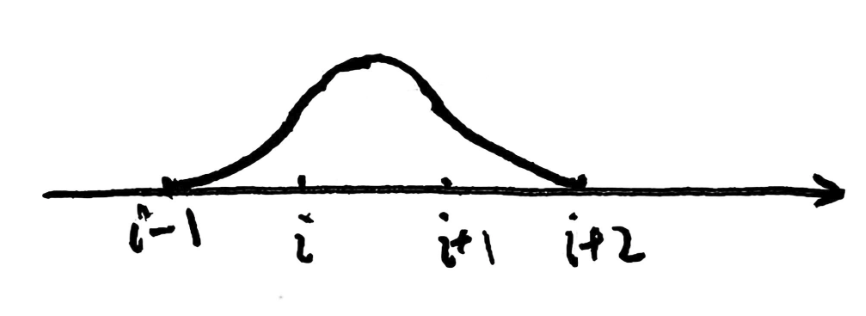
\includegraphics[width=0.8\textwidth]{Image1.png}
    \label{fig1}
\end{figure}

\section*{VI. Theorem 3.32}

\begin{align*}
  &(t_{i+2} - t_{i-1})[t_{i-1}, t_i, t_{i+1}, t_{i+2}](t - x)_+^2 \\
  =&(t_{i+2} - t_{i-1})\dfrac{[t_i, t_{i+1}, t_{i+2}] - [t_{i-1}, t_i, t_{i+1}]}{t_{i+2} - t_{i-1}}(t - x)_+^2 \\
  =&[t_i, t_{i+1}, t_{i+2}] (t - x)_+^2 - [t_{i-1}, t_i, t_{i+1}] (t - x)_+^2\\
  =&\dfrac{[t_{i+1}, t_{i+2}](t - x)_+^2 - [t_i, t_{i+2}](t - x)_+^2 - [t_{i-1}, t_{i+1}] (t - x)_+^2 + [t_{i-1}, t_i](t - x)_+^2}{t_{i+1} - t_{i}} \\
  =&\dfrac1{t_{i+1} - t_i}\left( \dfrac{(t_{i+2} - x)_+^2 - (t_{i+1} - x)_+^2}{t_{i+2} - t_{i+1}} - \dfrac{(t_{i+2} - x)_+^2 - (t_{i} - x)_+^2}{t_{i+2} - t_{i}} -\dfrac{(t_{i+1} - x)_+^2 - (t_{i-1} - x)_+^2}{t_{i+1} - t_{i-1}} + \dfrac{(t_{i-1} - x)_+^2 - (t_{i} - x)_+^2}{t_{i-1} - t_{i}} \right)\\
  =& 
\begin{cases}
\frac{(x - t_{i-1})^2}{(t_{i+1} - t_{i-1})(t_i - t_{i-1})}, & x \in (t_{i-1}, t_i] \\
\frac{x - t_{i-1}}{t_{i+1} - t_{i-1}} \cdot \frac{t_{i+1} - x}{t_{i+1} - t_i} + \frac{t_{i+2} - x}{t_{i+2} - t_i} \cdot \frac{x - t_i}{t_{i+1} - t_i}, & x \in (t_i, t_{i+1}] \\
\frac{(t_{i+2} - x)^2}{(t_{i+2} - t_i)(t_{i+2} - t_{i+1})}, & x \in (t_{i+1}, t_{i+2}] \\
0, & \text{otherwise}
\end{cases}\\
  =&B_i^2(x)
\end{align*}

\section*{VII. Scaled Integral of B-splines}

Define $K_i^n(x) = \dfrac{1}{t_{i+n} - t_{i-1}} \int_{t_{i-1}}^{t_{i+n}} B_i^n(x) \mathrm{d}x$

We use the theorem on derivatives of B-splines

$$\dfrac{\mathrm{d}}{\mathrm{d}x}B_i^n(x) = \dfrac{nB_i^{n-1}(x)}{t_{i+n-1} - t_{i-1}} - \dfrac{nB_{i+1}^{n-1}(x)}{t_{i+n} - t_{i}}$$

Integrating both sides over $\mathbb{R}$, we obtain:

$$\int_{t_{i-1}}^{t_{i+n}}\dfrac{\mathrm{d}}{\mathrm{d}x}B_i^n(x) \mathrm{d}x = \int_{t_{i-1}}^{t_{i+n-1}} \dfrac{nB_i^{n-1}(x)}{t_{i+n-1} - t_{i-1}} \mathrm{d}x - \int_{t_{i}}^{t_{i+n}} \dfrac{nB_{i+1}^{n-1}(x)}{t_{i+n} - t_{i}}$$

Since \( B_i^n(x) \) is compactly supported, the left-hand side is zero. Thus,
\[
0 = \frac{n}{t_{i+n} - t_i} \int_{-\infty}^{\infty} B_i^{n-1}(x)  dx - \frac{n}{t_{i+n+1} - t_{i+1}} \int_{-\infty}^{\infty} B_{i+1}^{n-1}(x)  dx,
\]
which implies
\[
K_i^{n-1}(x) = K_{i+1}^{n-1}(x)
\]

So $K_i^n(x)$, which is the scaled integral of a B-spline $B_i^n(x)$ over its support, is independent of the index $i$.

\section*{VIII. Symmetric Polynomials}

\subsection*{VIII-a}

The theorem states that for any positive integer \( m \), any integer \( i \), and any \( n = 0, 1, \ldots, m \), the complete symmetric polynomial can be expressed as a divided difference:
\[
\tau_{m-n}(x_i, \ldots, x_{i+n}) = [x_i, \ldots, x_{i+n}] x^m.
\]

We verify this for \( m = 4 \) and \( n = 2 \). Then \( m - n = 2 \), and we consider variables \( x_i, x_{i+1}, x_{i+2} \). The complete symmetric polynomial of degree 2 in three variables is:
\[
\tau_2(x_i, x_{i+1}, x_{i+2}) = x_i^2 + x_i x_{i+1} + x_i x_{i+2} + x_{i+1}^2 + x_{i+1} x_{i+2} + x_{i+2}^2.
\]

Now compute the divided difference \( [x_i, x_{i+1}, x_{i+2}] x^4 \). Let \( a = x_i \), \( b = x_{i+1} \), \( c = x_{i+2} \) for simplicity. The divided difference is defined recursively:
\[
[a, b, c] x^4 = \frac{ [b, c] x^4 - [a, b] x^4 }{ c - a }.
\]

First, compute the first-order divided differences:
\[
[a, b] x^4 = \frac{b^4 - a^4}{b - a} = a^3 + a^2 b + a b^2 + b^3,
\]
\[
[b, c] x^4 = \frac{c^4 - b^4}{c - b} = b^3 + b^2 c + b c^2 + c^3.
\]

Then,
\[
[a, b, c] x^4 = \frac{ (b^3 + b^2 c + b c^2 + c^3) - (a^3 + a^2 b + a b^2 + b^3) }{ c - a } = \frac{ b^2 c + b c^2 + c^3 - a^3 - a^2 b - a b^2 }{ c - a }.
\]

Let \( M = b^2 c + b c^2 + c^3 - a^3 - a^2 b - a b^2 \). Since \( M \) vanishes when \( a = c \), \( c - a \) is a factor. Polynomial division of \( M \) by \( c - a \) yields:
\[
\frac{M}{c - a} = a^2 + a b + a c + b^2 + b c + c^2.
\]

Thus,
\[
[a, b, c] x^4 = a^2 + a b + a c + b^2 + b c + c^2 = \tau_2(a, b, c).
\]

Therefore, the theorem holds for \( m = 4 \) and \( n = 2 \).

\subsection*{VIII-b}

We aim to prove the identity:
\[
\tau_{m-n}(x_i, \ldots, x_{i+n}) = [x_i, \ldots, x_{i+n}] x^m,
\]
using the recursive relation:
\[
\tau_{k+1}(x_1, \ldots, x_n, x_{n+1}) = \tau_{k+1}(x_1, \ldots, x_n) + x_{n+1} \tau_k(x_1, \ldots, x_n, x_{n+1}). \tag{3.54}
\]

We proceed by induction on \( n \).

\subsubsection*{Base Case: \( n = 0 \)}

Then the left-hand side is:
\[
\tau_{m}(x_i) = x_i^m,
\]
since the complete symmetric polynomial in one variable is just that variable raised to the power \( m \). The right-hand side is:
\[
[x_i] x^m = x_i^m.
\]
Thus, the identity holds for \( n = 0 \).

\subsubsection*{Inductive Step}

Assume the identity holds for all indices up to \( n-1 \), i.e.,
\[
\tau_{m-(n-1)}(x_j, \ldots, x_{j+n-1}) = [x_j, \ldots, x_{j+n-1}] x^m
\]
for any valid \( j \). Now consider \( n \) points: \( x_i, \ldots, x_{i+n} \). By the recursive definition of divided differences:
\[
[x_i, \ldots, x_{i+n}] x^m = \frac{ [x_{i+1}, \ldots, x_{i+n}] x^m - [x_i, \ldots, x_{i+n-1}] x^m }{ x_{i+n} - x_i }.
\]

By the inductive hypothesis:
\[
[x_{i+1}, \ldots, x_{i+n}] x^m = \tau_{m-n+1}(x_{i+1}, \ldots, x_{i+n}),
\]
\[
[x_i, \ldots, x_{i+n-1}] x^m = \tau_{m-n+1}(x_i, \ldots, x_{i+n-1}).
\]

Substituting these into the divided difference expression:
\[
[x_i, \ldots, x_{i+n}] x^m = \frac{ \tau_{m-n+1}(x_{i+1}, \ldots, x_{i+n}) - \tau_{m-n+1}(x_i, \ldots, x_{i+n-1}) }{ x_{i+n} - x_i }.
\]

Now, we use the recursive relation for complete symmetric polynomials. Consider the identity:
\[
(x_{n+1} - x_1) \tau_k(x_1, \ldots, x_{n+1}) = \tau_{k+1}(x_2, \ldots, x_{n+1}) - \tau_{k+1}(x_1, \ldots, x_n),
\]
which can be derived from (3.54). Let \( k = m-n \), and take the variables to be \( x_i, x_{i+1}, \ldots, x_{i+n} \). Then:
\[
(x_{i+n} - x_i) \tau_{m-n}(x_i, \ldots, x_{i+n}) = \tau_{m-n+1}(x_{i+1}, \ldots, x_{i+n}) - \tau_{m-n+1}(x_i, \ldots, x_{i+n-1}).
\]

Therefore:
\[
[x_i, \ldots, x_{i+n}] x^m = \frac{ (x_{i+n} - x_i) \tau_{m-n}(x_i, \ldots, x_{i+n}) }{ x_{i+n} - x_i } = \tau_{m-n}(x_i, \ldots, x_{i+n}).
\]

This completes the induction.

% \section*{ \center{\normalsize {Acknowledgement}} }
% Give your acknowledgements here(if any).


% \printbibliography

% If you are not familiar with \texttt{bibtex}, 
% it is acceptable to put a table here for your references.
\end{document}